\documentclass[12pt,letterpaper]{article}
\usepackage[utf8]{inputenc}
\usepackage[english]{babel}
\usepackage[left=1in,right=1in,top=1in,bottom=1in]{geometry}
\renewcommand*\familydefault{\sfdefault}
\usepackage{amsmath}
\usepackage{amsfonts}
\usepackage{amssymb}
\usepackage{graphicx}

\usepackage{subcaption}

\usepackage{pgf,tikz}
\usepackage{mathrsfs}
\usetikzlibrary{arrows}

\usepackage{listings}

\definecolor{darkgreen}{rgb}{0,0.5,0}
\definecolor{orange}{rgb}{1,0.5,0}
\lstset{language=C,
basicstyle=\ttfamily\scriptsize,
directivestyle=\color{red},
keywordstyle=\color{blue},
commentstyle=\color{darkgreen},
stringstyle=\color{orange},
breaklines=true,
mathescape}

\title{Quadtree/Octree Distribution of Data using p4est}
\author{Ana C. Perez-Gea}
\date{May 11, 2017}
\begin{document}
\maketitle

In this project we see the advantages of using mesh refinement to process massive amounts of data. When there are a large number of data points that a computer needs to process, it can be problematic when the computer does not have enough memory to load and process all data points at the same time. In this project I simulate a large number of data points and use quadtrees or octrees to partition the data and have different processors working with different parts of the data.  In particular, I use the package p4est in the C programming language to do the mesh refinement and load data into different processors.

\section{Data}

I simulated the data using a file of the NYU logo as seen in Figure \ref{nyu_logo}. I will cover the 2-dimensional case in detail and then extend the explanations to the 3-dimensional case. Inside of the torch, many points are generated and outside just a few. The $x$-coordinates of the figure are stored in one vector and the $y$-coordinates in another. At each image point, we repeat the storing of the row ($x$-coordinate) and column ($y$-coordinate) location of that data point but with random noise added each time. This is that for image row $i$ we loop for $0\leq j< m_i$ such that \[x_{i,j} = r_i + u_{i,j}\] where $u_{i,j}$ is a uniform random variable between 0 and 1 and $m_i$ is the number of repetitions for that image point. If we are at an inside point we repeat more times so $m_i$ will be larger than if we are at an outside point.

\begin{figure}[h]
\centering
\caption{Image for Data Simulation}
\label{nyu_logo}

\includegraphics[width=.3\textwidth]{NYU_logo}
\end{figure}

\section{p4est}

The package p4est does all the handling of the splitting of the quadtrees and octrees for us. I took the example file p4est\_step1.c and modified it for my purposes. In particular, it has a function that defines the condition for splitting. This function is a boolean that, if we have more than a certain number of points in a quadrant, will return 1.

\section{Quadtree}

I first implemented the 2-dimensional case. In table \ref{data} we can see the minimum and maximum row and column values as well as the total number of points generated for a single run. Since positive noise was added to the row and column values, we can see that the values go a little over zero or the number of rows and columns corresponding to the minimums and maximums respectively.

\begin{table}
\centering
\caption{Data}
\label{data}
\begin{tabular}{rl}
Min row:& 0.000008\\
Max row:& 397.999939\\
Min col:& 0.000289\\
Max col:& 406.000000\\
Total points: & 8001102
\end{tabular}
\end{table}

I ran the code using 5 processors with MPI and it took about 35 seconds. Figure \ref{quad_levels} shows the levels of partitioning. The red in the middle shows small areas and the blue outside shows large quadtrees. Figure \ref{quad_rank} shows the points that are being processed by the different processors. Each color represents a different processor, an MPI rank.

\begin{verbatim}
mpirun -np 5 p4est_data
\end{verbatim}

\begin{figure}[ht]
\centering
\caption{Quadtree}
\label{quadtree}
\begin{subfigure}[b]{0.45\textwidth}
\caption{Levels}
\label{quad_levels}
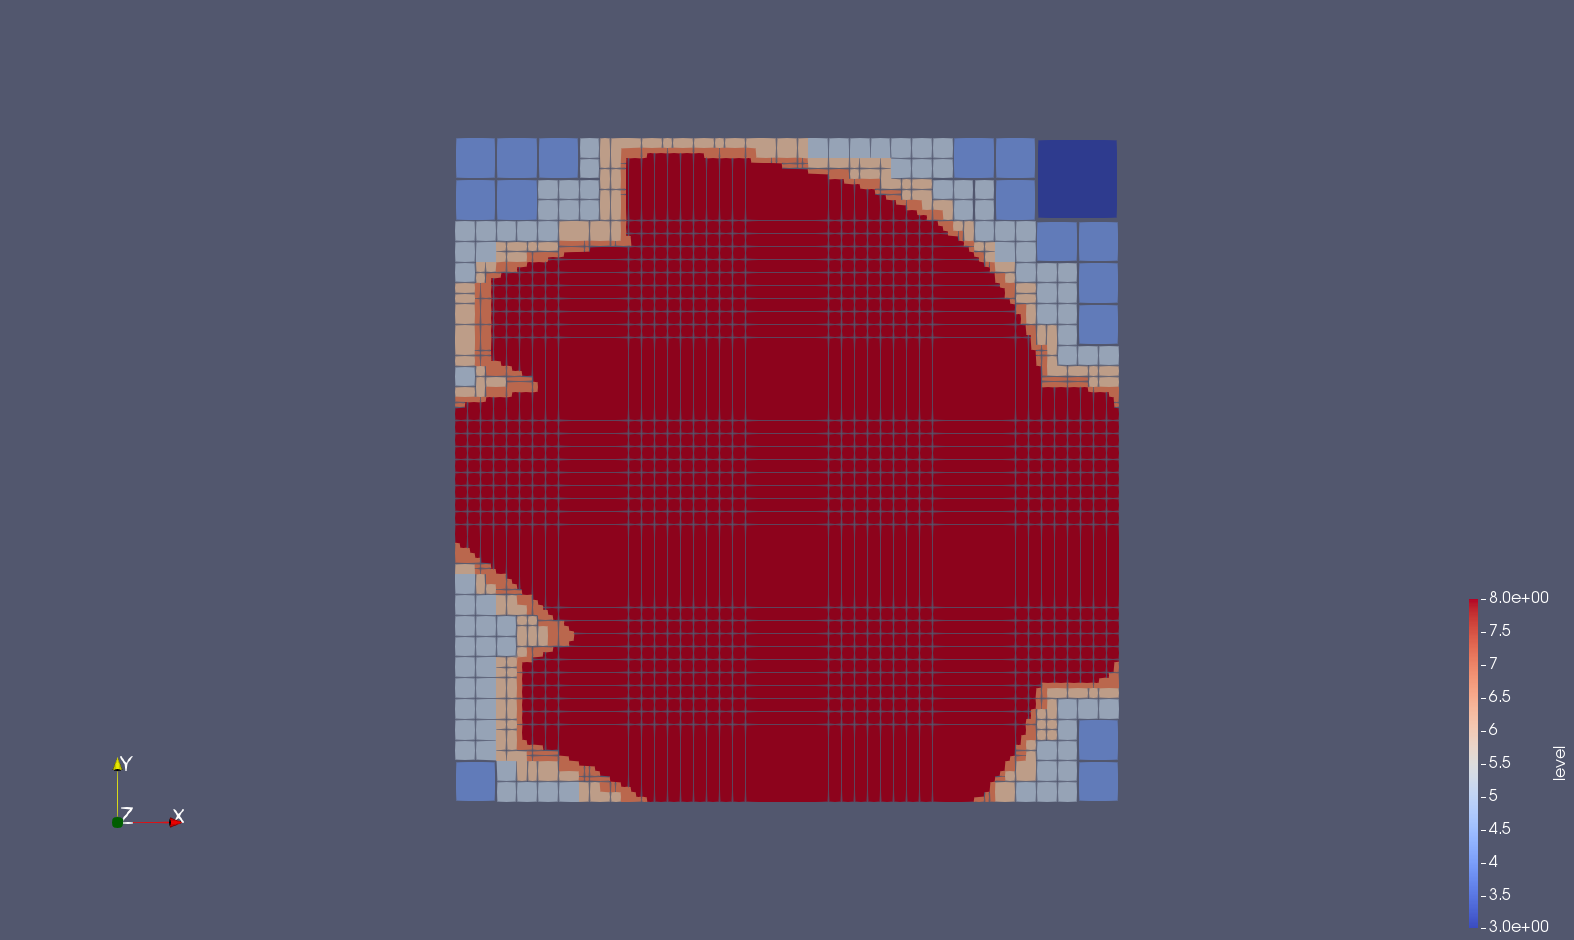
\includegraphics[width=\textwidth]{quad_level.png}
\end{subfigure}
\begin{subfigure}[b]{0.45\textwidth}
\caption{Rank}
\label{quad_rank}
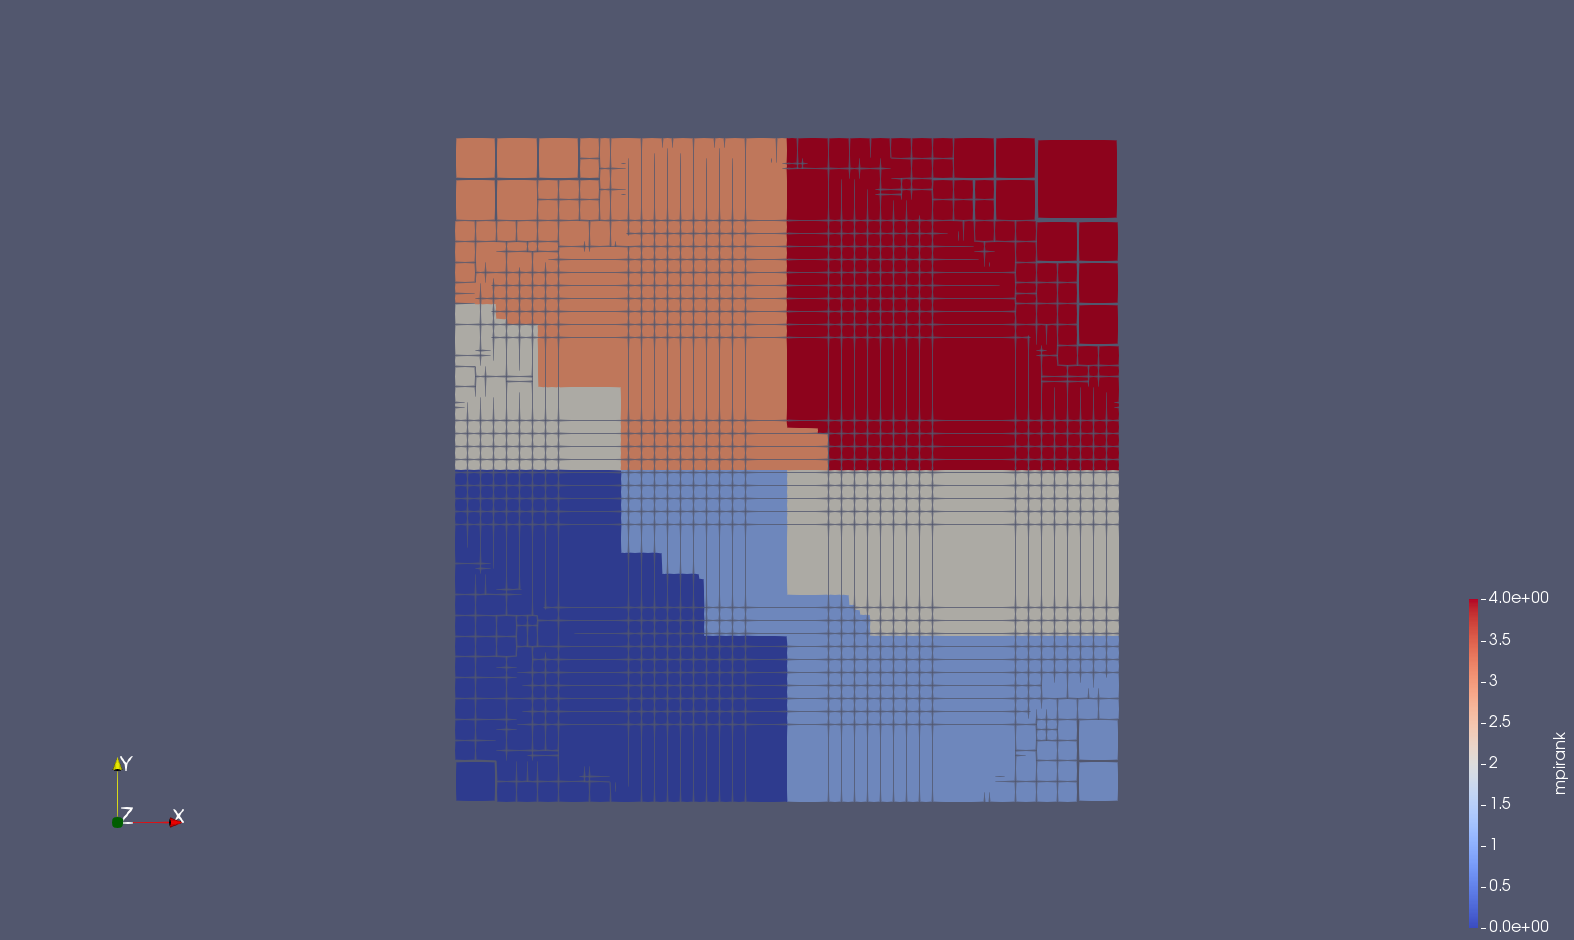
\includegraphics[width=\textwidth]{quad_rank.png}
\end{subfigure}
\end{figure}

\section{Octree}

Octrees are 3-dimensional representation of the quadtrees. In my case, I repeated the data in the $z$-direction 5/8 of the way up and 5/8 down. I repeated the above run with 5 MPI ranks for this 3-dimensional case. Now Figure \ref{octree} shows the data points themselves to be able to view the shape of the volume. We can see in Figure \ref{oct_levels} the levels of refinement by color. The red in the center is fine grid and the blue in the outside is coarse. In Figure \ref{oct_rank} the colors represent a different rank, where we can see each processor got about the same number of points.


\begin{verbatim}
mpirun -np 5 p8est_data
\end{verbatim}

\begin{figure}[ht]
\centering
\caption{Octree}
\label{octree}
\begin{subfigure}[b]{0.45\textwidth}
\caption{Levels}
\label{oct_levels}
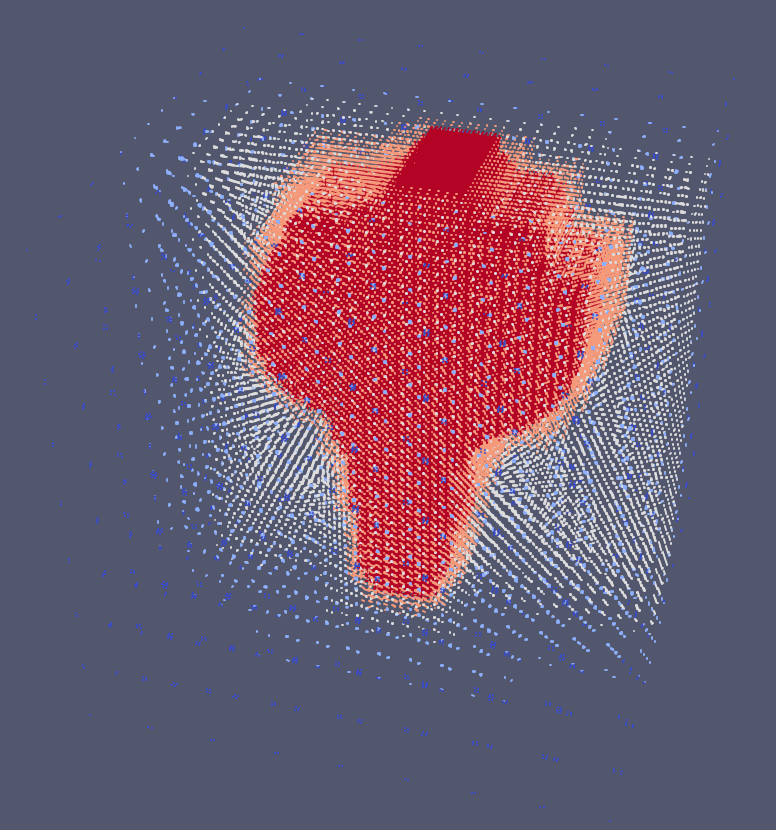
\includegraphics[width=\textwidth]{oct_level.png}
\end{subfigure}
\begin{subfigure}[b]{0.45\textwidth}
\caption{Rank}
\label{oct_rank}
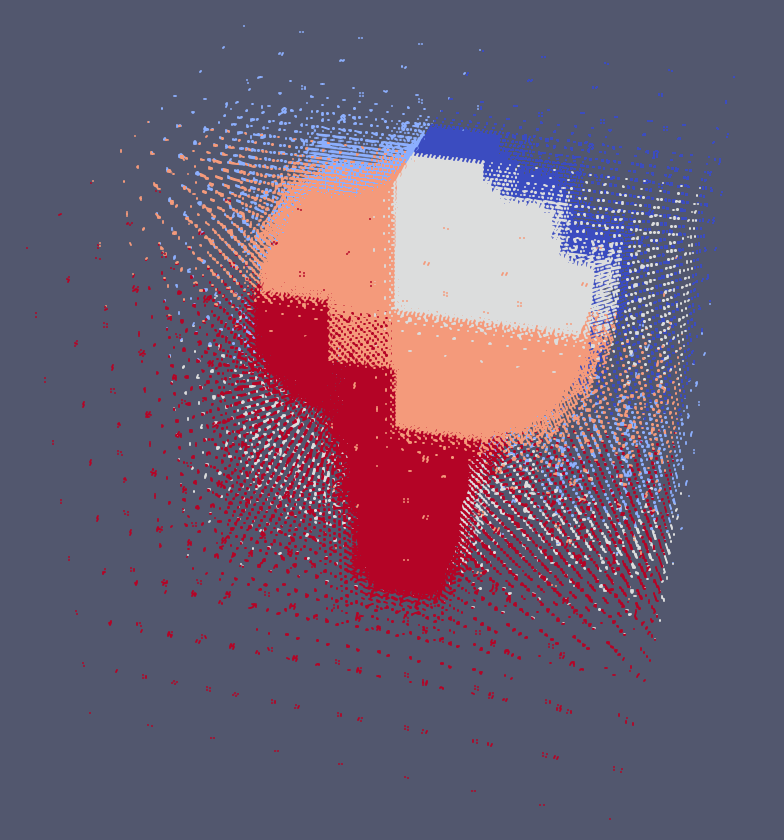
\includegraphics[width=\textwidth]{oct_rank.png}
\end{subfigure}
\end{figure}

\section{C Code}

\lstinputlisting{p4est_data.c}

\end{document}